%----------------------------------------------------------------
%
%  File    :  appendix.tex
%
%  Authors :  Keith Andrews, IICM, TU Graz, Austria
%             Manuel Koschuch, FH Campus Wien, Austria
% 
%  Created :  22 Feb 96
% 
%  Changed :  30 Oct 2008
%  !TEX root = ./thesis.tex
%----------------------------------------------------------------
\renewcommand*{\lstlistlistingname}{Codeverzeichnis}
\chapter{Anhang/Ergänzende Information}
\label{chap:app}
	% \begin{figure}[h!]
	% 	\centering
	% 	\begin{subfigure}
	% 		\centering
	% 		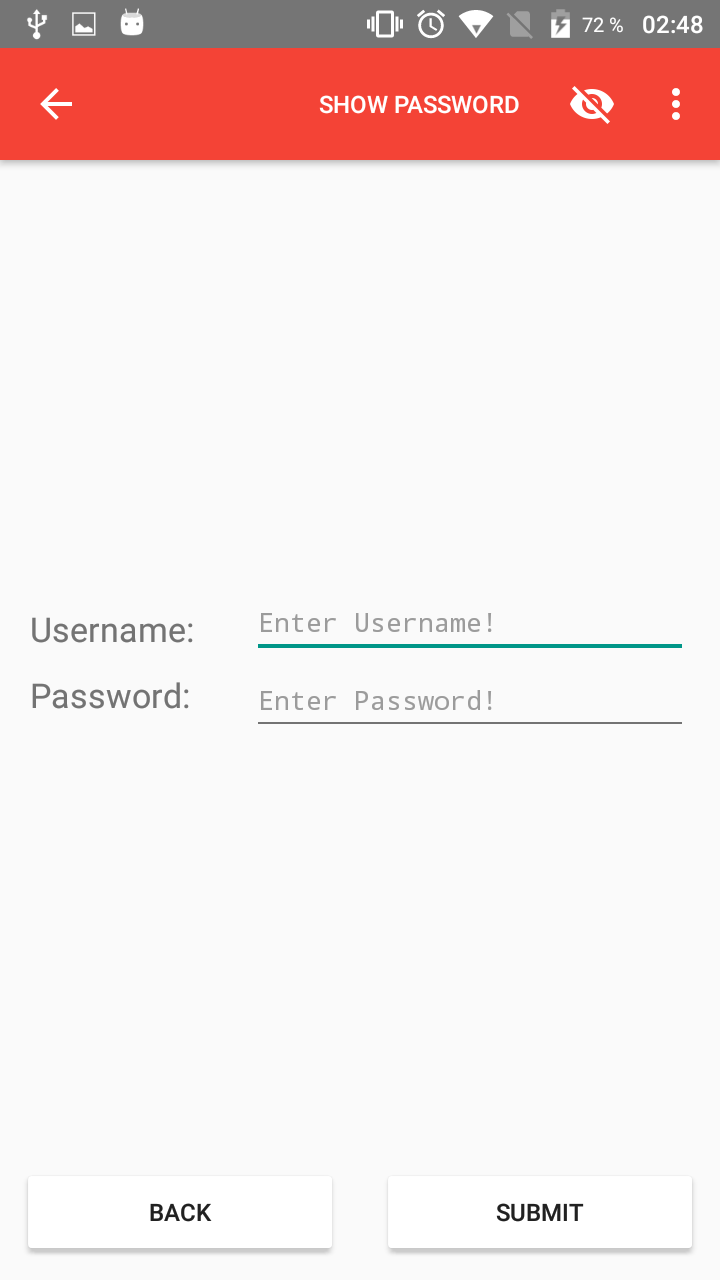
\includegraphics[width=.3\textwidth]{images/stm32kb-loginscreen.png}
	% 	\end{subfigure}
	% 	\label{fig:nope}
	% \end{figure}
	\begin{figure}[h!]
		\centering
		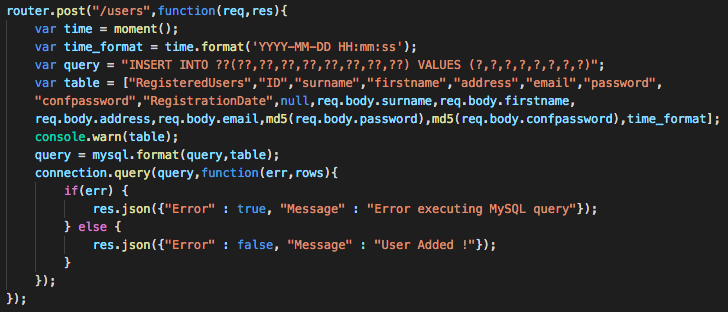
\includegraphics[width=1\textwidth]{images/restfull-server-code.png}
		\caption{RESTful - Server code - User Anlegen}
		\label{fig:serversidecode}
	\end{figure}

% section zusätzliche_screenshots (end)



% (Hier können Schaltpläne, Programme usw. eingefügt werden.)
% Hier werden die Entwürfe zur Design der App gelistet sein.b
\clearpage

% --- List of Figures ----------------------------------------------------

\addcontentsline{toc}{section}{Abbildungsverzeichnis}
\listoffigures

\clearpage

% --- List of Tables -----------------------------------------------------

\addcontentsline{toc}{section}{Codeverzeichnis}
\lstlistoflistings

\addcontentsline{toc}{section}{Tabellenverzeichnis}
\listoftables

\clearpage

% --- Bibliography ------------------------------------------------------

\bibliographystyle{alpha}


% List references I definitely want in the bibliography,
% regardless of whether or not I cite them in the thesis.

\nocite{book:Xamarin.Forms-Succinctly}
\nocite{book:Xamarin.Forms-Essentials:}
\nocite{book:Cross-platform-UI-Development-with-Xamarin.Forms}
\nocite{book:Xamarin-Mobile-Application-Development}
\nocite{Amer2016}
\nocite{Oleksandr2015}
\nocite{8016193}
\nocite{Mukesh2016}
\nocite{Soylemez2017}
\nocite{Maximilian2017}

\addcontentsline{toc}{section}{Literaturverzeichnis}
\bibliography{thesis}

